 %!TEX root = ./template-skripsi.tex
%-------------------------------------------------------------------------------
%                            BAB II
%               KAJIAN TEORI
%-------------------------------------------------------------------------------

\chapter{KAJIAN PUSTAKA} 

\section{Citra Gambar Digital}

Sebuah gambar dapat diberikan definisi sebagai fungsi dua dimensi \(f(x, y)\), 
dimana x dan y mewakili koordinat ruang (bidang) dan amplitudo f pada setiap 
pasangan koordinat \((x, y)\) merujuk pada intensitas atau level keabuan citra pada 
koordinat tersebut. Jika x, y, dan nilai intensitas f semuanya terbatas \emph{(finite)} 
dan memiliki nilai diskret, maka gambar tersebut dianggap sebagai gambar digital. 

Dalam hal ini, fungsi \emph{f(s, t)} merujuk pada fungsi gambar kontinu dengan dua variabel 
kontinu s dan t. Fungsi ini kemudian diubah menjadi gambar digital melalui proses \emph{sampling} 
dan kuantisasi. Melalui proses ini, sampel-sampel dari gambar kontinu diubah menjadi 
gambar digital \(f(x, y)\). Gambar digital dapat direpresentasikan dalam 
bentuk matriks \emph{(array)} yang terdiri dari nilai-nilai numerik \(f(x, y)\).

\begin{equation} \label{eq:array_citra}
  f(x,y) = 
  \begin{bmatrix}
    f(0,0) & f(0,1) & \cdots & f(0, N-1)\\
    f(1,0) & f(1,1) & \cdots & f(1, N-1)\\
    \vdots & \vdots & \vdots & \vdots\\
    f(M-1,0) & f(M-1,1) & \cdots & f(M-1,N-1)
  \end{bmatrix}
\end{equation}

Matriks \emph{(array)} diatas adalah representasi yang digunakan dalam pengolahan 
komputer (\cite{Gonzalez:2018}), dimana

\begin{conditions}
  f(x,y) & Fungsi gambar citra digital\\
  M & Banyaknya baris\\
  N & Banyaknya kolom\\
  x & 0, 1, 2, . . . , M - 1\\
  y & 0, 1, 2, . . . , N - 1
\end{conditions}

Sebuah citra digital merupakan sejumlah elemen yang memiliki batasan \emph{(finite)}, 
dan setiap elemen ini memiliki nilai dan posisi tertentu. Setiap elemen dari array 
ini disebut sebagai elemen gambar, elemen citra, piksel, atau pel. Piksel-piksel 
tertentu merepresentasikan nilai-nilai dalam array yang terletak pada pasangan 
koordinat (\(x,y\)) yang tetap. Piksel merupakan istilah yang paling umum digunakan 
untuk merujuk pada elemen-elemen citra digital (\cite{Gonzalez:2018}).

\section{Pemrosesan Citra Digital}
Pemrosesan gambar digital adalah proses yang dilakukan pada citra sebagai masukan
dengan melalui beberapa tahapan seperti pra-pemrosesan citra tersebut, mengekstrak 
(memsegmentasi) elemen, mendeskripsikan elemen dalam bentuk yang sesuai 
untuk pemrosesan citra tersebut.

\cite{Gonzalez:2018} menyebutkan bahwa pemrosesan citra digital dapat dikelompokkan 
menjadi tiga tingkatan, yakni rendah, menengah, dan tinggi. Pada tingkat pengolahan 
rendah, dilakukan operasi dasar seperti pra-pemrosesan citra guna mengurangi \emph{noise}, 
mempertajam kontras, serta memperjelas citra. Proses ini memfokuskan pada citra 
sebagai input maupun outputnya. Pengolahan tingkat menengah pada citra melibatkan 
langkah-langkah seperti membagi citra menjadi wilayah atau objek (segmentasi), 
menguraikan objek dalam citra untuk disesuaikan dengan pemrosesan komputer, dan 
mengenali objek secara keseluruhan. Pengolahan tingkat menengah ditandai oleh 
masukan yang umumnya berupa citra, dengan hasil keluaran berupa atribut yang 
diekstraksi dari citra tersebut (contohnya, tepi, kontur, dan identitas objek).
Akhirnya, pada tingkat pengolahan citra yang lebih tinggi, terdapat pengenalan 
objek dalam citra.

\section{Citra Gambar Berwarna}

\cite{Gonzalez:2018} dalam bukunya mengatakan bahwa Warna yang kita lihat pada objek 
dipengaruhi oleh cahaya yang dipantulkannya. Cahaya terlihat terdiri dari spektrum 
sempit dalam spektrum elektromagnetik. Objek yang memantulkan cahaya merata pada 
semua panjang gelombang terlihat putih, sementara yang memantulkan dalam rentang 
tertentu terlihat berwarna. Contohnya, objek hijau memantulkan cahaya dengan panjang 
gelombang 500-570 nm, menyerap pada panjang gelombang lainnya.

\begin{figure}[H]
	\centering{}
	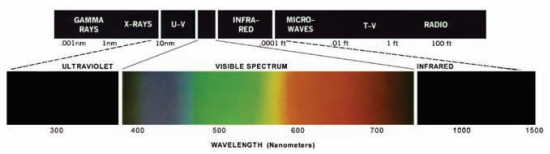
\includegraphics[width=\textwidth]{gambar/gelombang_cahaya.png}
	\caption{Spektrum cahaya, (\cite{Gonzalez:2018})}
\end{figure}

Mata manusia memiliki sel kerucut yang sensitif terhadap warna. Sekitar 65\% sensitif 
terhadap merah, 33\% terhadap hijau, dan hanya 2\% terhadap biru. Meskipun jarang, 
sel biru sangat sensitif. Sel-sel ini menyerap cahaya dengan karakteristik berbeda, 
sehingga mata kita melihat warna dengan gabungan merah (R), hijau (G), dan biru (B).

\begin{figure}[H]
	\centering{}
	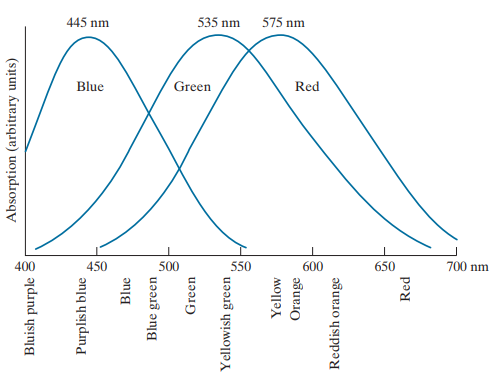
\includegraphics[width=0.8\textwidth]{gambar/gelombang_rgb_mata.png}
	\caption{Penyerapan cahaya yang ditangkap oleh mata dalam bentuk panjang gelombang, (\cite{Gonzalez:2018})}
\end{figure}

CIE menetapkan standar warna pada 1931, tetapi data eksperimental yang lebih akurat 
muncul pada 1965. Standar CIE hanya sekitar cocok dengan data eksperimental. 
Standar ini menetapkan panjang gelombang biru = 435,8 nm, hijau = 546,1 nm, dan 
merah = 700 nm sebagai warna primer.

Citra gambar yang direpresentasikan kedalam model warna RGB terdiri dari tiga bagian 
yang mewakili warna dasar: merah, hijau, dan biru. Ketika gambar ini ditampilkan di 
layar, ketiga bagian ini bergabung untuk membentuk gambar berwarna. Kita menyebutnya 
model warna RGB karena ini adalah singkatan dari \emph{Red} (merah), \emph{Green} 
(hijau), dan \emph{Blue} (biru). Setiap bagian gambar ini memerlukan sejumlah "bit" 
(ini seperti blok kecil yang menyimpan informasi), dan jumlah bit yang digunakan 
untuk setiap bagian piksel ini disebut "kedalaman piksel". Jika kita memiliki gambar 
RGB dengan setiap bagian (merah, hijau, dan biru) menggunakan 8 bit, maka setiap 
"piksel warna" dalam gambar ini (yang memiliki tiga nilai, satu untuk merah, satu 
untuk hijau, dan satu untuk biru) akan menggunakan total 24 bit (8 bit untuk merah + 
8 bit untuk hijau + 8 bit untuk biru).

\begin{figure}[H]
	\centering{}
	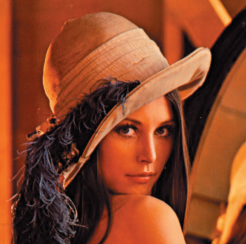
\includegraphics[width=0.4\textwidth]{gambar/gambar_citra_warna.png}
	\caption{Gambar citra berwarna, (\cite{Gonzalez:2018})}
\end{figure}

Gambar berwarna penuh sering disebut gambar RGB 24-bit. Ini artinya setiap piksel 
dalam gambar memiliki 24 bit untuk menyimpan informasi warnanya. Jumlah total warna 
yang bisa direpresentasikan dalam gambar RGB 24-bit sangat besar, sekitar 16 juta 
warna yang berbeda (\cite{Gonzalez:2018}).

\begin{figure}[H]
	\centering{}
	
\includegraphics[width=0.4\textwidth]{gambar/rgb_cube.png}
	\caption{24 bit kubus warna RGB, (\cite{Gonzalez:2018})}
\end{figure}

Untuk citra gambar digital, rentang nilai dalam kubus diukur dalam angka yang dapat 
direpresentasikan oleh jumlah bit dalam gambar. Jika, seperti di atas, gambar utama 
adalah gambar 8-bit, batas kubus sepanjang setiap sumbu menjadi [0, 255]. 
Sebagai contoh, warna putih akan berada pada titik [255, 255, 255] dalam kubus.

\section{Pemodelan Distribusi \emph{Gaussian Mixture Model}}

GMM (\emph{Gaussian Mixture Model}) adalah sebuah metode statistik yang dapat digunakan 
untuk memodelkan data sebagai kombinasi beberapa distribusi Gauss. Metode ini 
digunakan dalam segmentasi gambar untuk memodelkan gambar dalam bentuk gabungan 
dari distribusi Gaussian. GMM digunakan untuk memperkirakan probabilitas piksel 
yang termasuk ke dalam objek yang ingin di-segmentasi dan probabilitas piksel 
yang termasuk ke dalam latar belakang. 

\cite{Power:2002} dalam penelitiannya mengatakan setiap piksel terhadap objek diberi \emph{state} dari himpunan \(K\), di mana \(K\) 
adalah jumlah konstan biasanya antara 3 dan 7, \cite{Rother:2004} memberikan nilai \(K = 5\) . Beberapa \emph{state} \(K\) mewakili 
objek latar belakang sedangkan sisanya dianggap sebagai objek depan. \(\omega_k = P(k), k = 1,2,...,K,\) yang menunjukkan 
probabilitas priori munculnya permukaan \(k\) dalam pandangan piksel yaitu:

\begin{equation} \label{eq:prior_probability}
  \Sigma_{k=1}^{K} \: \omega_k = 1
\end{equation}
dimana, 

\begin{conditions}
  K & Parameter konstanta\\
  \omega_k & Probabilitas priori
\end{conditions}

Proses yang menghasilkan \emph{state} permukaan \(k\) tidak dapat di amati langsung dan hanya 
dapat di amati secara tidak langsung melalui nilai piksel terkait X. Bahkan jika 
kita tahu permukaan k yang sedang dilihat, nilai piksel masih memiliki distribusi 
\(f(X|k)\) karena faktor-faktor seperti perubahan pencahayaan, noise kamera, atau 
tekstur permukaan. Nilai piksel merupakan sampel dari variabel acak X yang mencakup 
perilaku k. X dapat berupa satu dimensi (intensitas monokrom), dua dimensi (ruang 
warna), tiga dimensi (warna), atau n-dimensi secara umum. 

peneliti membuat ilustrasi dari parameter gaussian dalam bentuk kurva yang berdistribusi 
normal dalam satu dimensi:

\begin{figure}[H]
	\centering{}
	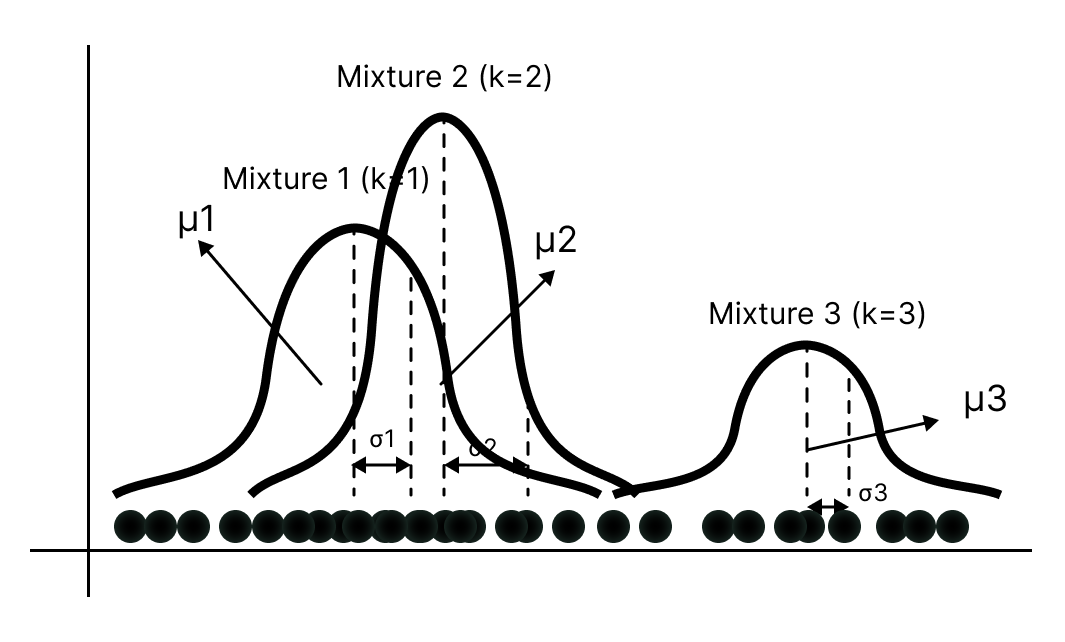
\includegraphics[width=0.8\textwidth]{gambar/gmm_curve.png}
	\caption{Contoh distribusi tiga fungsi gaussian 1 dimensi dengan parameter K = 3, (\cite{Power:2002})}
\end{figure}

Terlihat bahwa terdapat tiga fungsi gaussian, dengan parameter K = 3. Setiap gaussian
menjelaskan data-data yang terdapat pada tiga \emph{mixture} yang ada. 

Untuk memecahkan masalah segmentasi latar depan, \emph{state} k yang paling mungkin 
diestimasi pada setiap waktu sampel \(t\) dari sekelompok observasi yang diambil dari X, 
beserta prosedur untuk membedakan antara \emph{state} latar depan dan latar belakang.

Proses nilai piksel X diasumsikan direpresentasikan oleh kombinasi dari K densitas 
Gaussian, masing-masing dengan parameter \(\theta_k\), di mana setiap \emph{state} 
\(k\) memiliki parameter sendiri, secara umum rumus distribusi normal didefinisikan 4
sebagai berikut :

\begin{equation} \label{eq:distribusi_normal}
f(x) = \frac{1}{\sigma \sqrt{2\pi}} e^{-0.5 \bigl(\frac{x - \mu}{\sigma} \bigr)^2}
\end{equation}

dimana, 

\begin{conditions}
  f(x) & Distribusi normal\\
  \sigma & Standar deviasi\\
  x & Nilai variabel bebas\\
  \mu & Rata-rata
\end{conditions}

Persamaan di atas merupakan rumus dari distribusi normal (gaussian) untuk 1 dimensi, 
dimana parameter yang digunakan adalah standar deviasi (\(\sigma\)). Sedangkan 
untuk distribusi gaussian n-dimensi maka digunakan persamaan berikut :

\begin{equation} \label{eq:distribusi_multi}
	f_{X|k} (X|k, \theta_k) = \frac{1}{(2\pi)^\frac{n}{2} |\Sigma_k|^\frac{1}{2}} e^{-\frac{1}{2} (X - \mu_k)^T \Sigma^{-1}_k (X - \mu_k)}
\end{equation}

dimana, 

\begin{conditions}
  f_{X|k} (X|k, \theta_k) & Distribusi normal multivariat\\
  \Sigma_k & Matriks kovarians\\
  X & Vektor variabel bebas\\
  \mu_k & Vektor rata-rata komponen ke-k
\end{conditions}

Rata-rata \(\mu_k\) dan matriks kovarian \(\Sigma_k\) dari densitas ke-k digunakan 
dalam rumus tersebut. Biasanya diasumsikan bahwa dimensi X adalah independen, yang 
memungkinkan \(\Sigma_k\) menjadi diagonal dan lebih mudah dibalik. Variansi \(\sigma^2k\) 
berdimensi-n sering digunakan untuk merepresentasikan \(\Sigma_k\) dengan n varians 
tersebut identik, artinya deviasi dalam berbagai dimensi dari ruang warna (seperti 
merah, hijau, dan biru) memiliki statistik yang sama. Meskipun skalar tunggal 
\(\sigma_k^2\) mungkin menjadi pendekatan yang wajar dalam ruang warna linear, 
namun mungkin tidak akurat dalam aplikasi lain. Ruang warna non-linear seperti hue, 
saturasi, dan nilai (\emph{value}), serta ruang yang menggabungkan berbagai kuantitas 
seperti intensitas dan jangkauan, memerlukan perhatian khusus karena setiap dimensi 
kemungkinan memiliki distribusi yang unik.

Set parameter untuk densitas didefinisikan sebagai \( \theta_k = {\mu_k, \sigma_k}\) 
untuk suatu nilai k, dan set lengkap parameter adalah \(\Phi = {\omega_1, ..., 
\omega_K, \theta_1, ..., \theta_K}\). Karena kejadian k saling eksklusif, distribusi 
X dapat direpresentasikan sebagai campuran Gaussian, di mana setiap Gaussian 
sesuai dengan suatu nilai k tertentu (seperti yang ditunjukkan pada Gambar 1). 
Hal ini dapat dinyatakan sebagai berikut: 

\begin{equation} \label{eq:jumlah_distribusi}
  f_X(X|\Phi) = \Sigma_{k=1}^K P(k) f_{X|k} (X|k,\theta_k)
\end{equation}

dimana, 

\begin{conditions}
  f_X(X|\Phi) & Jumlah distribusi gaussian\\
  P(k) & Distribusi priori\\
\end{conditions}

di mana \(P(k) = \omega_k\). Semua parameter \(\Phi\), termasuk probabilitas P(k) dan parameter 
dari setiap Gaussian, harus diestimasi dari observasi X, sambil secara simultan 
memperkirakan keadaan tersembunyi k.

Setiap gaussian pada \(k\) terdiri dari beberapa parameter di antaranya sebagai berikut :

\begin{enumerate}
	\item Rata-rata \(\mu\) yang menginterpretasikan posisi titik puncak dari kurva
	\item Matriks kovarians \(\Sigma\) yang menginterpretasikan sebagai lebar kurva
	\item Probabilitas prior \(\omega\) merupakan peluang sebuah data berasal dari 
		suatu \emph{mixture} tertentu dengan jumlah maksimal sama dengan 1
\end{enumerate}

Dengan diasumsikan bahwa terdapat K distribusi yang dapat menghasilkan sampel X, 
probabilitas posterior \(P(k|X,\Phi)\) mewakili probabilitas bahwa nilai piksel termasuk 
dalam state k, yang diberikan oleh teorema Bayes: 

\begin{equation} \label{teorema_bayes}
	P(k|X,\Phi) = \frac{\omega_k f_{X|k} (X|k,\theta_k)}{f_X(X|\Phi)}
\end{equation}

dimana, 

\begin{conditions}
  P(k|X,\Phi) & Probabilitas posterior
\end{conditions}

Probabilitas ini dihitung dengan menggabungkan probabilitas prior P(k) dengan \emph{likelihood} 
\(f_{X|k}(X|k,\theta_k)\) dan \emph{likelihood} total \(f_X(X|\Phi)\). Nilai k yang memaksimalkan \(f_X(X|\Phi)\) 
adalah estimasi MAP (maximum a posteriori) k ini dapat dihitung menggunakan rumus:

\begin{equation} \label{maximum_posteriori}
  \begin{aligned}
    k & = arg \max_k P(k|X,\Phi) \\
      & = arg \max_k \omega_k f_{X|k} (X|k,\theta_k)
  \end{aligned}
\end{equation}
dimana, 

\begin{conditions}
  arg \max_k & Nilai k yang membuat \(P(k|X,\Phi)\) menjadi maksimum
\end{conditions}

Dengan \(f_X(X|\Phi)\) dalam persamaan (\ref{teorema_bayes}) tidak tergantung pada k.
Setelah memperoleh nilai k, selanjutnya menduga parameter GMM menggunakan metode
\emph{maximum likelihood} untuk memaksimumkan fungsi \emph{likelihood}, dimana rumus 
fungsi \emph{likelihood} adalah sebagai berikut:

\begin{equation} \label{}
	P(X_1, X_2, ..., X_N, k | \Phi) = \Pi_{t=1}^N \omega_k f_{X|k}(X_t|k,\theta_k)
\end{equation}



Adapun parameter penduga yang memaksimumkan persamaan di atas adalah sebagai berikut :

\begin{equation} \label{eq:omega}
	\hat{\omega_k} = \frac{1}{N} \Sigma_{t=1}^N P(k|X_t,\Phi)
\end{equation}

\begin{equation} \label{eq:mu}
	\hat{\mu} = \frac{\Sigma_{t=1}^N X_t P(k|X_t,\Phi)}{\Sigma_{t=1}^N P(k|X_t,\Phi)} 
\end{equation}

\begin{equation} \label{eq:sigma}
	\hat{\Sigma_k} = \frac{\Sigma_{t=1}^N ((X_t - \hat{\mu_k}) \cdot (X_t - \hat{\mu_k})) P(k|X_t,\Phi)}{\Sigma_{t=1}^N P(k|X_t,\Phi)}
\end{equation}

dimana, 

\begin{conditions}
  \hat{\omega_k} & Penduga maksimum dari \(\omega_k\)\\
  \hat{\mu} & Penduga maksimum dari \(\mu\)\\
  \hat{\Sigma_k} & Penduga maksumum dari \(\Sigma_k\)
\end{conditions}

% Dengan memisalkan rumus \ref{eq:rumus_energi1} dengan \(U = - \log P(X_1, X_2, ..., X_N, k | \Phi)\)
% maka didapatkan hasil seperti langkah kedua dari gambar \ref{img:2.6} yaitu 
% sebagai berikut :

% \begin{equation} \label{eq:phi}
% 	\hat{\Phi} = arg \min_{\Phi} P(k|X_t,\Phi)
% \end{equation}


\section{Segmentasi Pemisahan Objek dari Latar Belakang dengan Algoritma \emph{GraphCut}}

Pendekatan segmentasi yang dilakukan Boykov dan Kolmogorov sebagai pondasi mengenai algoritma 
\emph{GrabCut} dijelaskan secara mendetail.


\subsection{{Metode Awal}}

Dalam penelitiannya \cite{Boykov:2004} menjelaskan bahwa Greig et al merupakan yang 
pertama kali menemukan bahwa algoritma \emph{min-cut/max-flow} dari optimasi kombinasi,
algoritma ini dapat digunakan untuk meminimalkan fungsi energi tertentu. 
Energi yang dibahas selanjutnya dapat direpresentasikan sebagai: 

\begin{equation} \label{eq:rumus_energi}
  E(L) = \sum_{p \in P}  D_{p}(L_{p}) + \sum_{(p,q) \in N} V_{p,q}(L_{p}, L_{q})
\end{equation} 

dimana, 

\begin{conditions}
  E(L) & \emph{Cost Function} ()\\
  D_{p}(L_{p}) & Data penalti, pelabelan dengan fungsi \emph{likelihood}\\
  V_{p,q}(L_{p}, L_{q}) & Interaksi potensial yaitu diskontinuitas antar piksel\\
  p & Piksel pada gambar \\
  P & Gambar citra digital
\end{conditions}

\(L = {{L_{p} |p \in P}}\) merupakan pelabelan dari gambar \(P\), \(D_{p}(\cdot)\) adalah 
fungsi data penalti, \(V_{p,q}\) adalah interaksi potensial, dan N adalah himpunan dari 
semua pasangan piksel sebelahnya. Contoh pelabelan gambar ditunjukkan pada Gambar 
\ref{img:pelabelan_citra}. Data pinalti \(D_{p}(\cdot)\) menunjukkan preferensi label dari setiap 
piksel berdasarkan intensitas yang di amati dan ditentukan oleh fungsi \emph{likelihood}. 
Interaksi potensial \(V_{p,q}\) mendorong koherensi spasial dengan memberi diskontinuitas 
antara piksel sebelahnya.

Greig membuat grafik dengan dua terminal, yang memungkinkan \emph{cost} \emph{minimum cut} 
grafik untuk menghasilkan pelabelan L biner yang optimal secara global dalam kasus 
model interaksi Potts seperti yang dijelaskan dalam persamaan \ref{eq:rumus_energi}. Sebelum ini, 
tidak mungkin untuk secara tepat meminimalkan energi seperti \ref{eq:rumus_energi}, dan 
algoritma iteratif seperti simulasi anil biasanya digunakan sebagai gantinya.
Terlepas dari keefektifannya, teknik \emph{graph cut} Greig et al. sebagian besar 
tidak diperhatikan selama hampir satu dekade. Hal ini terutama disebabkan oleh 
fakta bahwa penerapannya dalam restorasi citra biner dianggap sangat terbatas. 
Awalnya, upaya untuk menggunakan algoritma \emph{graph cut} kombinatorial dalam 
\emph{computer vision} sebagian besar difokuskan pada pengelompokan gambar. Namun, 
pada akhir 1990-an, sejumlah besar teknik \emph{computer vision} baru muncul, 
yang mendemonstrasikan bagaimana algoritma \emph{min-cut/max-flow} dapat diterapkan 
pada graf untuk memecahkan-masalah non-biner yang lebih kompleks. 


\begin{figure}[H] 
\centering
  \begin{subfigure}{.5\textwidth}
    \centering{}
    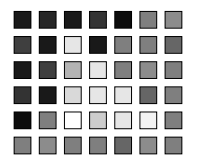
\includegraphics[width=0.55\textwidth]{gambar/gambar_1-A.png}
    \caption{Sebuah gambar}
  \end{subfigure}%
  \begin{subfigure}{.5\textwidth}
    \centering{}
    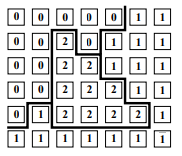
\includegraphics[width=0.55\textwidth]{gambar/gambar_1-B.png}
    \caption{Sebuah label}
  \end{subfigure}  
\caption{
    Contoh pelabelan gambar. citra (a) adalah himpunan piksel P dengan intensitas teramati Ip untuk setiap \(p \in P.\) Pelabelan L yang ditunjukkan 
    pada (b) memberikan beberapa label Lp ∈ {0, 1, 2} untuk setiap piksel \(p \in P.\) 
    } (\cite{Boykov:2004})
\label{img:pelabelan_citra}
\end{figure}


Pada gambar ditunjukkan bahwa \emph{graph} dengan tepi berbobot dapat digunakan untuk 
meminimalkan fungsi energi dengan hukuman interaksi linier dalam kasus multi-label. 
Konstruksi \emph{graph} ini telah diperluas untuk menangani klik cembung dan interaksi 
metrik. Metode yang disebut algoritma ekspans-\(\alpha\) menemukan solusi perkiraan 
dengan menjalankan algoritma \emph{min-cut/max-flow} pada \emph{graph} yang sesuai. 
Pendekatan ini dapat menangani berbagai macam klik, termasuk yang disukai dalam 
aplikasi praktis. Studi terbaru telah mengeksplorasi sifat teoritis konstruksi 
\emph{graph} yang digunakan dalam penglihatan. Sebuah studi mengidentifikasi kondisi 
yang diperlukan dan cukup untuk fungsi energi yang dapat diminimalkan menggunakan 
\emph{graph cut}. Namun, penelitian tersebut hanya berlaku untuk fungsi energi 
dengan variabel biner dan klik ganda atau tripel. Potensi penuh teknik \emph{graph cut} 
dalam kasus multi-label belum sepenuhnya dipahami

Sifat-sifat segmen yang dibuat dengan metode \emph{graph cut} diperiksa dalam 
sebuah penelitian yang disebutkan [3]. Penelitian ini berfokus pada metrik potongan 
yang diterapkan pada kisi \emph{graph} dan menunjukkan bahwa topologi diskrit dari 
\emph{graph cut} dapat meniru ruang metrik Riemannian secara kontinu. Penelitian 
dilakukan yang ada telah menciptakan hubungan antara dua pendekatan umum yang 
digunakan untuk meminimalkan energi: metode \emph{graph cut} kombinatorial 
dan metode geometris yang mengandalkan \emph{set level}.


\subsection{{Latar Belakang Pada Graf}}

Graf berbobot dan berarah, dilambangkan dengan \(G = \langle V, \varepsilon \rangle \) 
terdiri dari kumpulan \emph{node} V dan sisi berarah E yang menghubungkannya. 
\emph{Node} ini biasanya mewakili fitur, seperti piksel atau voxel. Graf juga 
menyertakan beberapa \emph{node} khusus yang dikenal sebagai terminal, yang sesuai 
dengan kemungkinan label yang dapat diberikan ke fitur, khususnya dalam konteks 
penglihatan. Pembahasan ini akan difokuskan pada graf yang hanya memiliki dua terminal.

\begin{figure}[H]
  \centering
    \begin{subfigure}{.5\textwidth}
      \centering{}
      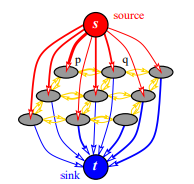
\includegraphics[width=0.55\textwidth]{gambar/graph-A.png}
      \caption{Sebuah graf \(G\)}
    \end{subfigure}%
    \begin{subfigure}{.5\textwidth}
      \centering{}
      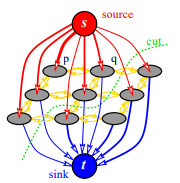
\includegraphics[width=0.55\textwidth]{gambar/cut-A.png}
      \caption{Sebuah potongan (\emph{cut}) \(G\)}
    \end{subfigure}  
  \caption{
    Contoh graf berkapasitas terarah. (\cite{Boykov:2004})
    }
  \label{img:graf_berarah}

\end{figure}

Terminal dalam \emph{graph} dikenal sebagai \emph{source} "s", dan \emph{sink}, "t." Contoh 
sederhana dari \emph{graph} dua terminal ditunjukkan pada Gambar \ref{img:graf_berarah}(a), yang dapat 
digunakan untuk meminimalkan energi Potts pada gambar \(3 x 3\) dengan dua label. 
Sebagian besar metode minimisasi energi dalam penglihatan didasarkan pada \emph{graph} 
grid 2D atau 3D biasa seperti yang ada pada Gambar \ref{img:graf_berarah}(a) karena simpul \emph{graph} biasanya 
mewakili piksel atau voxel gambar biasa. Setiap sisi dalam \emph{graph} memiliki bobot 
atau \emph{cost}, dan \emph{cost} sisi berarah \((p, q)\) mungkin berbeda dari \emph{cost} sisi sebaliknya 
\((q, p)\). Penting untuk dapat menetapkan bobot tepi yang berbeda untuk \((p, q)\) dan 
\((q, p)\) di banyak aplikasi berbasis \emph{graph} dalam penglihatan. \emph{Graph} biasanya terdiri 
dari dua jenis sisi: \emph{n-link} dan \emph{t-link}. \emph{N-link} menghubungkan piksel atau voxel 
yang bertetangga dan merepresentasikan sistem ketetanggaan dalam gambar. \emph{cost} 
\emph{n-link} sesuai dengan penalti untuk diskontinuitas antara piksel, yang berasal dari 
istilah interaksi piksel \(V_{p,q}\) dalam energi (\ref{eq:rumus_energi}). \emph{T-link} menghubungkan piksel 
dengan terminal (label), dan \emph{cost} \emph{t-link} yang menghubungkan piksel dan terminal 
sesuai dengan penalti untuk menetapkan label yang sesuai ke piksel, yang berasal 
dari istilah data \(D_{p}\) dalam energi (\ref{eq:rumus_energi}).

\subsubsection{Permasalahan pada \emph{Min-Cut} dan \emph{Max-Flow}} 

Sebuah \emph{Cut} pada graf dengan dua terminal, dinotasikan sebagai s/t, adalah 
pemisahan \emph{node} dalam graf menjadi dua himpunan bagian yang terpisah dan 
tidak tumpang tindih, S dan T. \emph{Source} (s), termasuk dalam himpunan bagian S, 
dan \emph{sink} (t), termasuk dalam subset T. Pemotongan s/t disebut sebagai \emph{cuts}. 
Contoh potongan ditunjukkan pada gambar \ref{img:graf_berarah} (b).

\begin{figure}[H]
  \centering
    \begin{subfigure}{0.3\textwidth}
      \centering{}
      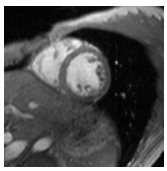
\includegraphics[width=\textwidth]{gambar/gambar-2.png}
      \caption{Gambar Awal}
    \end{subfigure}%
    \begin{subfigure}{0.3\textwidth}
      \centering{}
      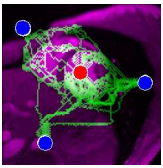
\includegraphics[width=\textwidth]{gambar/gambar-2a.png}
      \caption{\emph{Maximum Flow}}
    \end{subfigure}  
    \begin{subfigure}{0.3\textwidth}
      \centering{}
      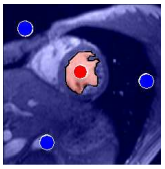
\includegraphics[width=\textwidth]{gambar/gambar-2b.png}
      \caption{\emph{Minimum Cut}}
    \end{subfigure}   
  \caption{
    Contoh (\emph{graph cut})/\emph{flow} dalam konteks segmentasi gambar. 
    (a) menunjukkan \emph{maximum flow} dari s ke t. Faktanya, ini menjenuhkan tepi 
    \emph{graph} yang sesuai dengan batas \emph{minimum cut} di (b). (\cite{Boykov:2004})
    }
    \label{img:contoh_flow}
\end{figure}
Dalam optimasi kombinatorial, \emph{cost} \emph{cut} \(C = {\mathcal{S,T}}\) didefinisikan sebagai 
jumlah \emph{cost} dari tepi batas (p, q) di mana \(p \in S\) dan \(q \in T\) . Perhatikan 
bahwa \emph{cost} \emph{cut} adalah "diarahkan" karena menjumlahkan bobot dari sisi-sisi 
yang diarahkan secara khusus dari \(\mathcal{S}\) ke \(\mathcal{T}\) . Masalah \emph{minimum cut}  pada 
graf adalah menemukan \emph{cut} yang memiliki \emph{cost} minimum di antara semua \emph{cut}. 

Salah satu konsep dasar dalam optimisasi kombinatorial adalah bahwa masalah mencari 
\emph{minimum cut} s/t dapat diselesaikan dengan menentukan \emph{maximum flow} dari 
\emph{source} s ke \emph{sink} t. Secara sederhana, \emph{maximum flow} mewakili 
"jumlah air" maksimum yang dapat diangkut dari sumber ke sumur dengan mempertimbangkan 
tepi graf sebagai pipa yang diarahkan dengan kapasitas yang sama dengan bobot tepinya. 
Menurut teorema Ford dan Fulkerson, \emph{maximum flow} dari s ke t mengisi sekelompok 
tepi di graf yang memisahkan simpul-simpul menjadi dua bagian yang tidak beririsan, 
\({S, T}\), yang sesuai dengan \emph{minimum cut}. Oleh karena itu, masalah 
\emph{minimum cut} dan \emph{maximum flow} adalah setara, dan nilai \emph{maximum flow} 
sama dengan \emph{cost} \emph{minimum cut}. Hubungan "dualitas" antara masalah \emph{maximum flow} 
dan \emph{minimum cut} diilustrasikan pada gambar \ref{img:contoh_flow} dalam konteks segmentasi gambar, 
di mana \emph{maximum flow} yang ditampilkan pada gambar \ref{img:contoh_flow}(a) mengisi 
tepi-tepi pada batas \emph{minimum cut} pada gambar \ref{img:contoh_flow}(b).

Konsep \emph{min-cut} atau \emph{max-flow} pada graf dapat digunakan untuk meminimalkan 
energi dalam pelabelan gambar. Jika kita memiliki gambar 3x3 dan menerapkan \emph{cut} 
s/t padanya, \emph{node} akan dibagi menjadi kelompok terpisah, masing-masing hanya 
berisi satu terminal. Pembagian ini mewakili penugasan piksel ke label. Dengan 
memberikan bobot tepat pada tepian berdasarkan parameter energi, kita dapat mencapai 
energi minimum dengan mencari pemotongan \emph{cost} minimum yang sesuai dengan 
pelabelan energi minimum.

% \subsubsection{Algoritma Standar dalam Optimasi Kombinatorial} \label{bagian:algoritma_standar}

% Fakta penting dalam optimasi kombinatorial adalah adanya algoritma polinomial untuk 
% masalah \emph{min cut/max-flow} pada graf berbobot terarah dengan dua terminal. Sebagian 
% besar algoritma termasuk dalam salah satu dari dua kelompok berikut: metode "\emph{push-relabel}" 
% gaya Goldberg-Tarjan dan algoritma berdasarkan \emph{augmenting path} gaya Ford-Fulkerson.


% Algoritma berbasis \emph{augmenting path} seperti algoritma Dinic bekerja dengan mencari jalur yang tidak jenuh 
% dari sumber ke tujuan dalam suatu graf dan mendorong aliran sepanjang jalur tersebut 
% hingga mencapai aliran maksimum. Algoritma \emph{augmenting path} menyimpan informasi 
% tentang distribusi aliran saat ini \(s \rightarrow t\) di antara tepi-tetapi graf 
% \(\mathcal{G}\) menggunakan graf residual \(\mathcal{G}_{f}\). Topologi 
% \(\mathcal{G}_{f}\) sama dengan \(\mathcal{G}\) tetapi kapasitas tepi di \(\mathcal{G}_{f}\) 
% mencerminkan kapasitas residu di tepi yang sama di \(\mathcal{G}\) dengan jumlah 
% aliran yang sudah ada di tepi tersebut. Pada awalnya, graf residual \( \mathcal{G}_{0} \) 
% tidak memiliki aliran (f=0) dan kapasitas tepi di graf residual \( \mathcal{G}_{0} \) 
% sama dengan kapasitas tepi di \(\mathcal{G}\). Pada setiap iterasi baru, algoritma menemukan 
% jalur \(s \rightarrow t\) terpendek di sepanjang tepi yang tidak jenuh di graf 
% residual \(\mathcal{G}_{f}\). Jika suatu jalur ditemukan, algoritma menambahkannya 
% dengan mendorong aliran maksimum yang mungkin \(df\) yang menjejali setidaknya satu 
% tepi dalam jalur tersebut. Kapasitas residu tepi dalam jalur dikurangi oleh \(df\) 
% sementara kapasitas residu tepi terbalik ditingkatkan oleh \(df\). Setiap penambahan 
% atau \emph{augmentation} eningkatkan total aliran dari sumber ke tujuan, yaitu \(f = f + df\). Aliran maksimum 
% tercapai ketika setiap jalur \(s \rightarrow t\) melintasi setidaknya satu tepi 
% jenuh di graf residual \(\mathcal{G}_{f}\).

% Algoritma Dinic menggunakan pencarian luas pertama untuk menemukan jalur terpendek
% dari \(s\) ke \(t\) pada graf residual \(\mathcal{G}_{f}\). Setelah semua jalur terpendek dengan panjang 
% tetap \(k\) jenuh, algoritma memulai pencarian pertama lebar untuk \(s \rightarrow t\) jalur dengan 
% panjang \(k + 1\) dari awal. Perhatikan bahwa penggunaan jalur terpendek merupakan 
% faktor penting yang meningkatkan kompleksitas waktu berjalan teoretis untuk algoritma 
% berdasarkan jalur augmentasi. Kompleksitas running time kasus terburuk untuk algoritma 
% Dinic adalah \(O(mn^2 )\) di mana \(n\) adalah jumlah \emph{node} dan \(m\) adalah jumlah sisi dalam graf.

% Algoritma \emph{push-relabel} berbeda dengan metode \emph{augmenting path} karena 
% tidak berfokus pada menjaga \emph{flow} yang valid selama operasi. Sebaliknya, mereka 
% mencatat \emph{node} aktif dengan kelebihan \emph{flow} positif dan memberikan perkiraan batas 
% bawah jarak ke \emph{sink} melalui edge yang belum jenuh. Tujuannya adalah untuk mendorong 
% \emph{flow} yang berlebihan ke \emph{node} dengan perkiraan jarak yang lebih kecil ke sink. 
% Operasi push biasanya diterapkan pada \emph{node} aktif dengan jarak terbesar atau berdasarkan 
% strategi seleksi FIFO. Saat operasi push jenuh, jarak (label) meningkat secara progresif. 
% \emph{Flow} yang tidak dapat disampaikan akhirnya dikembalikan ke \emph{source}.


\subsection{{Algoritma \emph{Mincut/Max-Flow} Terbaru}}


Untuk meningkatkan performa empiris teknik augmenting path standar pada graf 
dalam \emph{computer vision}, \cite{Boykov:2004} mengembangkan algoritma baru. Biasanya, 
metode \emph{augmenting path} memulai pencarian lebar baru untuk jalur \(s \rightarrow t\) 
segera setelah semua jalur dari panjang tertentu habis. Namun, membangun pohon 
pencarian lebar untuk graf dalam \emph{computer vision} melibatkan pemindaian sebagian 
besar piksel gambar, sehingga menjadi operasi yang mahal jika dilakukan terlalu 
sering. Eksperimen dengan data nyata dalam \emph{computer vision} mengonfirmasi bahwa 
membangun kembali pohon pencarian menghasilkan kinerja yang buruk dari teknik 
\emph{augmenting path} standar. Untuk mengatasi masalah ini, \cite{Boykov:2004} 
mengembangkan beberapa ide yang meningkatkan performa empiris teknik \emph{augmenting path} 
pada graf dalam \emph{computer vision}.


\begin{figure}[H]
  \centering
  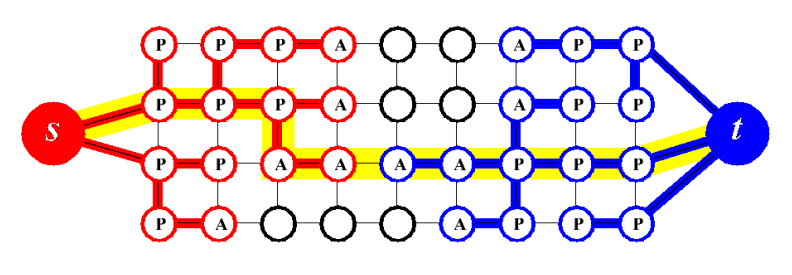
\includegraphics[width=0.8\textwidth]{gambar/gambar-3.png}
  \caption{
    Contoh pencarian pohon \(S\) (\emph{node} merah) dan \(T\) (\emph{node} biru) (\cite{Boykov:2004})
    }
  \label{img:contoh_pencarian_pohon}
\end{figure}

Algoritma min-cut/max-flow baru yang disajikan di sini termasuk dalam kelompok 
algoritma berdasarkan \emph{augmenting path}. Seperti algoritma Dinic, algoritma 
yang dibuat oleh \cite{Boykov:2004} juga membuat pohon pencarian untuk mendeteksi 
jalur pembesaran. Namun, membuat dua pohon pencarian, satu dari \emph{source} dan satu 
lagi dari \emph{sink}. Menggunakan kembali pohon-pohon ini dan tidak membuatnya 
dari awal setiap kali. Salah satu kelemahan pendekatan algoritma ini adalah jalur 
pembesaran yang ditemukan tidak selalu merupakan jalur pembesaran terpendek, sehingga 
kompleksitas waktu untuk menemukan jalur pembesaran terpendek tidak lagi valid. 
Jumlah maksimum penambahan yang dapat dilakukan oleh algoritma, dibatasi oleh 
biaya \emph{minimum cut} \(|C|\), sehingga kompleksitas waktu terburuknya adalah
\(O(mn^2 |C|)\).

\subsubsection{Penjelasan Algoritma} 

\cite{Boykov:2004} mempertahankan dua pohon pencarian yang tidak tumpang tindih 
\(S\) dan \(T\) dengan akar pada \emph{source} s dan \emph{sink} t, secara berurutan. 
Pada pohon S semua sisi dari setiap \emph{node} induk ke anaknya tidak jenuh, sedangkan 
pada pohon T sisi dari anak ke induknya tidak jenuh. \emph{node} yang tidak ada di S atau T 
disebut "bebas".

\begin{equation} \label{eq:status_node}
  S \subset V, s \in S, T \subset V, t \in T, S \cap T = 0
\end{equation} 

\emph{Node} dalam pohon pencarian \(S\) dan \(T\) dapat berupa "aktif" atau "pasif". \emph{node} 
aktif mewakili batas luar di setiap pohon sedangkan \emph{node} pasif adalah internal. 
Intinya adalah \emph{node} aktif memungkinkan pohon untuk "tumbuh" dengan memperoleh 
anak baru (sepanjang tepi yang tidak jenuh) dari sekumpulan \emph{node} bebas. 
\emph{node} pasif tidak dapat tumbuh karena sepenuhnya diblokir oleh \emph{node} 
lain dari pohon yang sama. Penting juga bahwa \emph{node} aktif dapat bersentuhan dengan 
\emph{node} dari pohon lain. Jalur augmentasi ditemukan segera setelah \emph{node} aktif 
di salah satu pohon mendeteksi \emph{node} tetangga yang dimiliki oleh pohon lainnya.


Algoritma secara iteratif mengulangi tiga tahap berikut:
\begin{itemize}
    \item Tahap “pertumbuhan atau (\emph{growth})”: cari pohon \(S\) dan \(T\) tumbuh hingga bersinggungan memberikan jalur \(s \rightarrow t\)  
    \item Tahap "augmentasi atau (\emph{augmentation})": jalur yang ditemukan ditambah, pohon pencarian dipecah menjadi hutan
    \item Tahap “adopsi atau (\emph{adoption})”: pohon \(S\) dan \(T\) dipulihkan.
\end{itemize}

% Pada tahap pertumbuhan atau (\emph{growth}), pohon pencarian berkembang dan \emph{node} 
% aktif mengeksplorasi tepi yang tidak jenuh dan memperoleh anak baru dari himpunan 
% \emph{node} bebas. Anak yang baru diperoleh menjadi anggota aktif dari pohon pencarian 
% yang sesuai. Ketika semua tetangga dari \emph{node} aktif telah dijelajahi, \emph{node} 
% aktif menjadi pasif. Tahap pertumbuhan berakhir ketika \emph{node} aktif menemukan 
% \emph{node} tetangga yang termasuk dalam pohon pencarian yang berlawanan, menandakan 
% bahwa telah ditemukan jalur dari \emph{source} ke \emph{sink}.

Pada tahap pertumbuhan (\emph{growth}), pohon pencarian berkembang dengan \emph{node} 
aktif mengeksplorasi tepi yang belum terjenuh dan mendapatkan anak baru dari himpunan 
\emph{node} bebas. Anak-anak baru ini menjadi bagian aktif dari pohon pencarian yang 
sesuai. Ketika semua tetangga dari \emph{node} aktif telah dijelajahi, status \emph{node} aktif 
berubah menjadi pasif. Tahap pertumbuhan berakhir ketika \emph{node} aktif menemukan 
tetangga yang sudah ada dalam pohon pencarian lawan, menunjukkan penemuan jalur dari 
\emph{source} ke \emph{sink}.

% Pada tahap augmentasi, jalur yang ditemukan pada tahap pertumbuhan ditambah dengan 
% mendorong aliran terbesar yang mungkin melalui jalur tersebut. Hal ini dapat 
% menyebabkan beberapa tepi menjadi jenuh, sehingga beberapa \emph{node} dalam pohon 
% \(S\) dan \(T\) menjadi "\emph{orphans}" karena tautan mereka ke induknya tidak lagi 
% valid. Tahap augmentasi juga dapat membagi pohon \(S\) dan \(T\) menjadi hutan.
% Namun, pada tahap adopsi atau (\emph{adoption}), tujuannya adalah untuk mengembalikan 
% struktur satu-pohon ke dalam himpunan \(S\) dan \(T\) dengan akar di \emph{source} 
% dan \emph{sink}. Ini dicapai dengan mencari induk baru yang valid untuk setiap 
% \emph{orphans} dalam himpunan yang sama, terhubung melalui tepi yang tidak jenuh. Jika 
% tidak ditemukan induk yang memenuhi syarat, \emph{orphans} dihapus dari \(S\) atau \(T\) 
% dan menjadi \emph{node} bebas, dan semua anak yang sebelumnya menjadi \emph{orphans}.

Pada tahap augmentasi, jalur yang ditemukan pada tahap pertumbuhan ditingkatkan 
dengan mengalirkan aliran maksimum melalui jalur tersebut. Ini bisa membuat beberapa 
tepi menjadi jenuh, mengakibatkan beberapa \emph{node} dalam himpunan \(S\) dan \(T\) menjadi 
\emph{"orphans"} karena tautan induk mereka tidak lagi valid. Tahap augmentasi juga bisa 
memisahkan pohon \(S\) dan \(T\) menjadi hutan.

Pada tahap adopsi, tujuannya adalah mengembalikan struktur satu-pohon ke dalam himpunan 
\(S\) dan \(T\) dengan akar di \emph{source} dan \emph{sink}. Ini dilakukan dengan mencari induk 
baru yang valid untuk setiap \emph{"orphans"} dalam himpunan yang sama, terhubung melalui 
tepi yang tidak jenuh. Jika tidak ditemukan induk yang memenuhi syarat, \emph{"orphans"} 
dihapus dari \(S\) atau \(T\), menjadi \emph{node} bebas, dan semua anak yang sebelumnya 
menjadi \emph{"orphans"}.

% Tahap adopsi atau \emph{adoption} terus berlanjut sampai semua \emph{orphans} telah menemukan induk 
% baru yang valid atau telah menjadi \emph{node} bebas. Proses ini akan memperkecil ukuran 
% \emph{set} \(S\) dan \(T\). Setelah tahap adopsi selesai, algoritma kembali ke tahap pertumbuhan. 
% Algoritma berakhir saat tidak ada lagi \emph{node} aktif tersisa dan pohon pencarian \(S\) dan \(T\) 
% terpisah oleh tepi yang jenuh, menunjukkan bahwa aliran maksimum telah dicapai. 
% Potongan minimum dapat ditentukan dengan menetapkan \(S\) dan \(T\) pada pohon yang sesuai.

Tahap adopsi \emph{(adoption)} berlanjut sampai semua \emph{"orphans"} telah menemukan 
induk baru yang valid atau telah menjadi \emph{node} bebas. Ini mengakibatkan pengurangan 
ukuran set \(S\) dan \(T\). Setelah tahap adopsi selesai, algoritma kembali ke tahap 
pertumbuhan. Algoritma berakhir saat tidak ada \emph{node} aktif yang tersisa dan pohon 
pencarian \(S\) dan \(T\) terisolasi oleh tepi yang jenuh, menunjukkan pencapaian 
aliran maksimum. Potongan minimum dapat ditentukan dengan menetapkan \(S\) dan \(T\) 
pada pohon yang sesuai.

\subsubsection{Implementasi Lebih Lanjut} 

Asumsikan bahwa kita memiliki graf berarah \(\mathcal{G = hV, Ei}\). Untuk setiap algoritma 
\emph{augmenting path}, kita akan mempertahankan aliran \(f\) dan graf residual \(Gf\) 
(lihat Bagian 2.1.2.2). Menyimpan daftar semua \emph{node} aktif, \(A\), dan semua \emph{orphans}, \(O\). 
Struktur umum algoritma adalah:

\begin{lstlisting} [label={pseudo:1.0}]
  initialize: (S = {s}, T = {t}, A = {s, t}, O = Ø)
  while true
      grow S or T to find an augmenting path P from s to t
      if P = Ø terminate
      augment on P
      adopt orphans
  end while  
\end{lstlisting}

Rincian tahap pertumbuhan, augmentasi, dan adopsi dijelaskan di bawah ini. Lebih 
mudah untuk menyimpan muatan dari pohon pencarian \(S\) dan \(T\) melalui \(flag\) \emph{TREE(p)} 
yang menunjukkan afiliasi dari setiap \emph{node} p sehingga

\begin{equation} \label{eq:searchtree_awal}
  TREE(p) =  \Biggl\{\begin{matrix}
    S & if & p & \in & S\\
    T & if & p & \in & T\\
    $\O$ & if & p & is & free
    \end{matrix}
\end{equation}

Jika \emph{node} p milik salah satu pohon pencarian maka informasi tentang induknya 
akan disimpan sebagai \(PARENT(p)\). Akar pohon pencarian (\emph{source} dan \emph{sink}), 
\emph{orphans}, dan semua \emph{node} bebas tidak memiliki orang tua, 
t.e. \emph{PARENT(p)} = Ø. Notasi \(tree\textunderscore cap(p \rightarrow q)\) 
untuk mendeskripsikan kapasitas residual dari salah satu sisi \((p, q)\) jika \(TREE(p) = S\) 
atau sisi \((q, p)\) jika \(TREE(p) = T\). Sisi-sisi ini harus tidak jenuh agar 
\emph{node} p menjadi orangtua yang valid dari anaknya q tergantung pada pohon pencarian.

\paragraph{Fase \emph{Growth}} \label{fase_growth}

Pada tahap ini node aktif memperoleh anak baru dari satu set node bebas.

\begin{lstlisting}
  while A $\neq$ Ø
    pick an active node $p \in A$
    for every neighbor q such that $tree\textunderscore cap(p \rightarrow q)$ > 0
    if $TREE(q) =$ Ø then add q to search tree 
    as an active node:
    $TREE(q) \neq TREE(p), PARENT(q) \neq p, A \neq A \cup \{q\}$
    if $TREE(q) \neq$ Ø and $TREE(q) \neq TREE(p)$ 
    return $P = PATH_{s \rightarrow t}$
    end for
    remove p from A
  end while
  return P = Ø
\end{lstlisting}


\paragraph{Fase \emph{Augmentation}} \label{fase_augmentation}

Input untuk tahap ini adalah jalur P dari s ke t. Perhatikan bahwa himpunan anak 
yatim kosong pada awal tahap, tetapi mungkin ada beberapa \emph{orphans} pada akhirnya 
karena setidaknya satu sisi di P menjadi jenuh.

\begin{lstlisting}
  find the bottleneck capacity $\Delta$ on P
  update the residual graph by pushing flow $\Delta$ through P
  for each \emph{edge} $(p, q)$ in P that becomes saturated
    if $TREE(p) = TREE(q)$ = S 
      then set $PARENT(q)$ := Ø and $O := O \cup {q}$
    if $TREE(p) = TREE(q)$ = T 
      then set $PARENT(p)$ := Ø and $O := O \cup {p}$
  end for
\end{lstlisting}


\paragraph{Fase \emph{Adoption}} \label{fase_adoption}

Selama tahap ini semua \emph{node} \emph{orphans} di O diproses sampai O menjadi kosong. 
Setiap \emph{node} p sedang diproses mencoba menemukan induk baru yang valid di dalam pohon 
pencarian yang sama; jika berhasil, p tetap berada di pohon tetapi dengan induk baru, 
jika tidak, ia menjadi \emph{node} bebas dan semua anaknya ditambahkan ke O.

\begin{lstlisting}
  while O $\neq$ Ø  
    pick an orphan node $p \in O$ and remove it from O
    process p
  end while
\end{lstlisting}

Operasi \emph{"proses p"} terdiri dari langkah-langkah berikut. Pertama kita mencoba mencari 
induk valid baru untuk \(p\) di antara tetangganya. Induk \(q\) yang valid harus memenuhi: 
\(TREE(q) = TREE(p)\), \(tree\textunderscore cap(q \rightarrow p) > 0\), dan “origin” 
dari \(q\) harus berupa \emph{source} atau c \emph{sink}. Perhatikan bahwa kondisi terakhir 
diperlukan karena selama tahap adopsi beberapa \emph{node} dalam pohon pencarian \(S\) atau \(T\) 
mungkin berasal dari \emph{orphans}. Jika \emph{node} \(p\) menemukan induk baru yang valid 
\(q\) maka kita atur \(PARENT(p) = q\). Dalam hal ini \(p\) tetap berada di pohon pencariannya 
dan status aktif (atau pasif) p tetap tidak berubah. 

Jika \(p\) tidak menemukan induk yang valid maka \(p\) menjadi \emph{node} bebas dan operasi 
berikut dilakukan:

\begin{itemize}
  \item Memindai semua tetangga q dari p sehingga TREE(q) = TREE(p):  
  \begin{itemize}
    \item jika \(tree\textunderscore cap(q \rightarrow p) > 0\) tambahkan q kepada set A yang aktif
    \item jika \(PARENT(q) = p\) tambahkan q kepada set \emph{orphans} O dan set \(PARENT(q) :=\) Ø
  \end{itemize}
  \item \(TREE(p) :=\) Ø, \(A := A - \{p\}\)
\end{itemize}

Perhatikan bahwa ketika \(p\) menjadi bebas, semua tetangganya yang terhubung melalui 
tepi yang tidak jenuh harus menjadi aktif. Mungkin saja beberapa tetangga \(q\) tidak 
memenuhi syarat sebagai orang tua yang valid selama tahap adopsi karena tidak berasal 
dari sumber atau sink. Namun, \emph{node} ini bisa menjadi induk yang valid setelah 
tahap adopsi selesai. Pada titik ini \(q\) harus berstatus aktif karena terletak di 
sebelah \emph{node} bebas \(p\).


\section{Segmentasi Citra dengan Algoritma \emph{GrabCut}}

% \cite{Rother:2004} melakukan penelitian mengenai segmentasi gambar dengan memanfaatkan 
% citra gambar, menyatakan bahwa alat segmentasi gambar klasik menggunakan salah satu 
% informasi tekstur (warna), misalnya. \emph{Magic Wand}, atau informasi tepi (kontras), 
% misalnya \emph{Intelligent Scissors}. \cite{Rother:2004} melakukan pendekatan yang didasarkan 
% pada pengoptimalan dengan \emph{GraphCut} telah dikembangkan yang berhasil menggabungkan 
% kedua jenis informasi tersebut.

% Ekstraksi interaktif dari objek latar depan dalam lingkungan kompleks yang latar 
% belakangnya tidak dapat dikurangkan dengan mudah. Tujuan dari algoritma ini adalah 
% untuk menghasilkan pemisahan objek dari latar belakang yang berkualitas tinggi, 
% sambil hanya memerlukan sedikit masukan dari pengguna. Output dari algoritma ini 
% adalah \emph{alpha-matte}, yang menunjukkan proporsi \emph{foreground} dan \emph{background} pada 
% setiap piksel.  Algoritma ini bertujuan untuk mencapai segmentasi objek yang akurat, 
% nilai alpha yang meyakinkan yang memperhitungkan blur, piksel campuran, dan transparansi, 
% serta warna \emph{foreground} yang bersih dan tidak terpengaruh oleh bleeding warna 
% dari latar belakang asli. Jumlah interaksi yang dibutuhkan dari pengguna dapat 
% bervariasi mulai dari mengedit piksel individu hingga hanya menandai beberapa lokasi 
% \emph{foreground} atau \emph{background}. 

Penelitian oleh \cite{Rother:2004} mengenai segmentasi gambar memanfaatkan citra 
dan menyatakan bahwa alat segmentasi gambar klasik menggunakan informasi tekstur 
(misalnya, warna) seperti \emph{Magic Wand}, atau informasi tepi (misalnya 
\emph{Intelligent Scissors}). Pendekatan yang digunakan oleh \cite{Rother:2004} 
berbasis pengoptimalan dengan \emph{GraphCut} dan berhasil menggabungkan kedua jenis 
informasi tersebut.

Tujuan algoritma ini adalah memisahkan objek dari latar belakang dalam lingkungan 
kompleks tanpa memerlukan banyak masukan pengguna. Hasilnya berupa alpha-matte yang 
menunjukkan proporsi \emph{foreground} dan \emph{background} pada setiap piksel. Algoritma ini 
bertujuan untuk memberikan segmentasi objek yang akurat, nilai alpha yang memperhitungkan 
blur, piksel campuran, transparansi, dan warna \emph{foreground} yang bersih tanpa 
terpengaruh oleh warna latar belakang. Jumlah interaksi pengguna dapat bervariasi, 
mulai dari mengedit piksel hingga menandai lokasi \emph{foreground} atau \emph{background}.

\subsection{{Sistem yang Diusulkan : \emph{GrabCut}}}

% Sebuah alat pemotongan gambar yang baik seharusnya dapat menghasilkan nilai alpha 
% yang halus di seluruh wilayah inferensi dari trimap, tanpa memberlakukan batasan 
% keras yang membatasi nilai alpha menjadi hanya 0 atau 1. Hal ini akan memungkinkan 
% untuk menangani secara otomatis masalah seperti asap, rambut, dan pohon. Namun, ini 
% menunjukkan bahwa teknik yang dirancang untuk memecahkan masalah 
% pemotongan gambar secara umum hanya efektif ketika terdapat cukup pemisahan antara 
% distribusi warna \emph{foreground} dan \emph{background}.

% Pertama kita memperoleh segmentasi “keras” menggunakan \emph{Graph Cut} iteratif. 
% Ini diikuti dengan \emph{matting} batas (bagian 4) di mana nilai \emph{alpha} dihitung dalam 
% jalur sempit di sekitar batas segmentasi keras. Terakhir, transparansi penuh, selain 
% di perbatasan, tidak ditangani oleh \emph{GrabCut} . Itu bisa dicapai namun menggunakan 
% \emph{matting brush} dan, ini bekerja dengan baik di area yang cukup bebas.

% Kebaruan pendekatan yang dilakukan Boykov pertama-tama terletak pada penanganan segmentasi. \cite{Boykov:2004} 
% telah membuat dua peningkatan pada mekanisme \emph{Graph Cut}: "estimasi iteratif" 
% dan "pelabelan tidak lengkap" yang memungkinkan tingkat interaksi pengguna yang 
% sangat berkurang untuk kualitas hasil tertentu (gambar \ref{img:2.5}(f)). Hal ini memungkinkan 
% \emph{GrabCut} untuk memberi beban ringan pada pengguna, yang interaksinya hanya 
% terdiri dari menyeret persegi panjang di sekitar objek yang diinginkan. Dengan 
% demikian, pengguna menunjukkan wilayah latar belakang, dan bebas dari kebutuhan 
% untuk menandai wilayah latar depan. Mereka juga telah mengembangkan mekanisme 
% baru untuk komputasi \emph{alpha}, yang digunakan untuk \emph{border matting}, di mana nilai 
% \emph{alpha} diatur untuk mengurangi artefak yang terlihat.

Alat pemotongan gambar yang baik harus menghasilkan nilai alpha yang halus di seluruh 
wilayah inferensi trimap, tanpa batasan keras 0 atau 1, untuk menangani masalah seperti asap, 
rambut, dan pohon. Teknik pemotongan gambar umumnya efektif saat ada pemisahan 
yang jelas antara distribusi warna \emph{foreground} dan \emph{background}.

Langkah pertama adalah segmentasi "keras" menggunakan \emph{Graph Cut} iteratif. 
Kemudian dilakukan matting batas di sekitar segmentasi keras, di mana nilai alpha 
dihitung dalam jalur sempit. Namun, GrabCut tidak menangani transparansi penuh 
selain di perbatasan, yang dapat dicapai dengan matting brush dalam area yang cukup bebas.

Pendekatan Boykov memperkenalkan peningkatan pada mekanisme \emph{Graph Cut}. Ini mencakup 
"estimasi iteratif" dan "pelabelan tidak lengkap" yang mengurangi interaksi pengguna. 
GrabCut memberikan kemudahan interaksi bagi pengguna dengan hanya menarik persegi 
panjang di sekitar objek. Mereka juga mengembangkan mekanisme baru untuk menghitung 
alpha dalam \emph{border matting} guna mengurangi artefak.


\subsection{{Segmentasi gambar dengan \emph{graph cut}}}

Segmentasi citra monokrom, diberi trimap awal T. Citra merupakan \emph{array} 
\(\textbf{z} = (z_{1},...,z_{n},...,z_{N})\) dengan nilai keabuan, diindeks dengan indeks (tunggal) n. 
Segmentasi gambar diekspresikan sebagai susunan nilai “opasitas” 
\(\alpha = (\alpha_{1},...,\alpha_{N})\) pada setiap piksel. Umumnya \( 0 \leq \alpha_{n} \leq 1\), 
tetapi untuk segmentasi keras \(\alpha_{n} \in {0,1}\), dengan 0 untuk latar belakang 
dan 1 untuk latar depan. Parameter \(\underline{\theta}\) menggambarkan distribusi 
tingkat keabuan latar depan dan latar belakang, dan terdiri dari histogram nilai 
keabuan: 

\begin{equation} \label{eq:2.4}
  \underline{\theta} = \{h(z;\alpha), \alpha = 0,1\}
\end{equation} 
dimana,
\begin{conditions}
  \theta & Distribusi tingkat keabuan dari gambar citra\\
  \alpha & Nilai alpha tiap piksel 1 untuk \emph{foreground} dan 0 untuk \emph{background}\\
  h & Histogram tingkat keabuan
\end{conditions}

satu untuk latar belakang dan satu untuk latar depan. Histogram dirakit langsung 
dari piksel berlabel dari masing-masing wilayah trimap \(T_{B},T_{F}\) . (Histogram dinormalisasi 
untuk dijumlahkan menjadi 1 pada rentang tingkat abu-abu: \(\int_{z} h(z;\alpha) = 1\).) Tugas 
segmentasi adalah menyimpulkan variabel opasitas yang tidak diketahui \(\alpha\) dari data 
gambar yang diberikan z dan model \(\theta\).

\subsubsection{{Segmentasi dengan \emph{energy minimisation}}}

Fungsi energi \textbf{E} didefinisikan pada persamaan \ref{eq:rumus_energi} yang dijelaskan oleh \cite{Boykov:2004} 
sehingga minimumnya harus sesuai dengan segmentasi yang baik, dalam arti bahwa ia dipandu baik oleh histogram 
tingkat abu-abu latar depan dan latar belakang yang di amati dan bahwa opasitasnya 
"koheren", yang mencerminkan kecenderungan soliditas objek. \cite{Rother:2004} 
menuliskan kembali energi "Gibbs" dalam bentuk:


\begin{equation} \label{eq:2.5}
  E(\underline{\alpha}, \underline{\theta}, \textbf{z}) = U(\underline{\alpha}, 
  \underline{\theta}, \textbf{z}) + V (\underline{\alpha}, \textbf{z})
\end{equation} 

dimana,
\begin{conditions}
  E & \emph{Cost Function} atau Rumus Energi \\
  U(\underline{\alpha}, \underline{\theta}, \textbf{z}) & Data penalti, seperti pada rumus \ref{eq:rumus_energi}\\
  V (\underline{\alpha}, \textbf{z}) & Interaksi potensial yaitu diskontinuitas antar piksel\\
  \textbf{z} & Nilai warna tiap piksel pada citra digital
  % \underline{\theta} & Model distribusi keabua 
\end{conditions}

Istilah data \(U\) mengevaluasi kecocokan distribusi opasitas \(\underline{\alpha}\) 
dengan data \textbf{z}, mengingat model histogram \(\underline{\theta}\), dan didefinisikan sebagai:

\begin{equation} \label{eq:2.6}
  U(\underline{\alpha}, \underline{\theta}, \textbf{z}) = \sum_{n} - \log h(z_{n};\alpha_{n}) 
\end{equation} 

dimana,
\begin{conditions}
  E & \emph{Cost Function} atau Rumus Energi \\
  U(\underline{\alpha}, \underline{\theta}, \textbf{z}) & Data penalti, seperti pada rumus \ref{eq:rumus_energi}\\
  % \underline{\alpha} & Nilai alpha \\
  % \underline{\theta} & Model distribusi keabua 
\end{conditions}

Istilah \emph{smoothness} dapat dituliskan sebagai :

\begin{equation} \label{eq:smoothness}
  V (\underline{\alpha}, \textbf{z}) = \gamma \sum_{(m,n) \in \textbf{C}} dis(m,n)^{-1}
  [\alpha_{n} \neq \alpha_{m}]exp - \beta(z_{m} - z_{n})^2
\end{equation} 

dimana,
\begin{conditions}
  E & \emph{Cost Function} atau Rumus Energi \\
  V (\underline{\alpha}, \textbf{z}) & Interaksi potensial yaitu diskontinuitas antar piksel\\
  \gamma & niai gamma \\
  m & Suatu piksel \\
  n & Tetangga dari piksel m \\
  \beta(z_{m} - z_{n})^2 & \emph{Beta smoothness}
\end{conditions}

di mana \([\phi]\) menunjukkan fungsi indikator yang mengambil nilai 0,1 untuk predikat 
\(\phi\), C adalah himpunan pasangan piksel tetangga, dan \(dis(\cdot)\) adalah jarak Euclidean 
piksel tetangga. Energi ini mendorong koherensi di wilayah dengan tingkat abu-abu 
yang serupa. Dalam praktiknya, hasil yang baik diperoleh dengan mendefinisikan 
piksel sebagai tetangga jika berdekatan baik secara horizontal/vertikal maupun 
diagonal (konektivitas 8 arah). Ketika konstanta \(\beta = 0\), istilah kehalusan 
hanyalah Ising sebelumnya yang terkenal, mendorong kehalusan di mana-mana, hingga 
tingkat yang ditentukan oleh konstanta \(\gamma\). Namun telah ditunjukkan bahwa 
jauh lebih efektif untuk mengatur \(\beta > 0\) karena hal ini mengurangi kecenderungan 
kehalusan di daerah dengan kontras tinggi. Konstanta \(\beta\) dipilih menjadi :

\begin{equation} \label{eq:2.8}
  \beta = \Bigl( 2 \bigl \langle (z_{m} - z_{n})^2 \bigl \rangle \Bigr)^{-1}
\end{equation} 

di mana \(\langle(\cdot)\rangle\) menunjukkan harapan atas sampel gambar. Pilihan 
\(\beta\) ini memastikan bahwa suku eksponensial dalam \ref{eq:smoothness} beralih dengan 
tepat antara kontras tinggi dan rendah. Konstanta \(\gamma\) diperoleh sebesar 50 
dengan mengoptimalkan kinerja terhadap kebenaran dasar melalui satu set pelatihan 
yang terdiri dari 15 gambar. Ini terbukti menjadi pengaturan serbaguna untuk berbagai 
macam gambar. Sekarang setelah model energi didefinisikan sepenuhnya, segmentasi 
dapat diperkirakan sebagai minimum global:

\begin{equation} \label{eq:2.9}
 \hat{\underline{\alpha}}  = arg \min_{\underline{\alpha}} \textbf{E}(\alpha,\theta).
\end{equation} 

Algoritma pemotongan minimum standar digunakan untuk minimisasi. Ini menjadi dasar 
bagi segmentasi keras, yang kemudian mengembangkan tiga perubahan untuk algoritma 
segmentasi dalam GrabCut. Pertama, model gambar monokrom digantikan oleh Model 
Campuran Gaussian (GMM) untuk warna. Kedua, estimasi \emph{one-shot minimum cut} 
diganti dengan prosedur iteratif lebih kuat yang bergantian antara estimasi dan 
pembelajaran parameter. Ketiga, permintaan pengguna interaktif dilemahkan, memungkinkan 
pelabelan yang tidak lengkap - pengguna hanya menentukan \(T_{B}\) untuk trimap, 
dengan cara menempatkan bentuk di sekitar objek.

\begin{figure}[H]
  \centering
    \begin{subfigure}{0.3\textwidth}
      \centering{}
      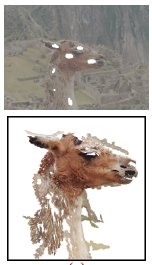
\includegraphics[width=\textwidth]{gambar/gambar-2_5(a).png}
      \caption{\emph{Magic Wand}}
    \end{subfigure}%
    \begin{subfigure}{0.3\textwidth}
      \centering{}
      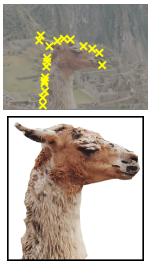
\includegraphics[width=\textwidth]{gambar/gambar-2_5(b).png}
      \caption{\emph{Intelligent Scissors}}
    \end{subfigure}  
    \begin{subfigure}{0.3\textwidth}
      \centering{}
      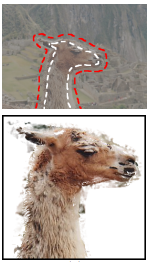
\includegraphics[width=\textwidth]{gambar/gambar-2_5(c).png}
      \caption{\emph{Bayes Matte}}
    \end{subfigure}  
    \begin{subfigure}{0.3\textwidth}
      \centering{}
      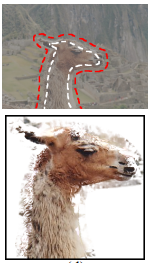
\includegraphics[width=\textwidth]{gambar/gambar-2_5(d).png}
      \caption{\emph{Knockout 2}}
    \end{subfigure}  
    \begin{subfigure}{0.3\textwidth}
      \centering{}
      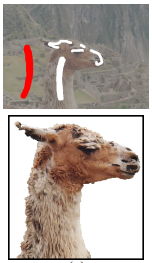
\includegraphics[width=\textwidth]{gambar/gambar-2_5(e).png}
      \caption{\emph{GraphCut}}
    \end{subfigure}   
    \begin{subfigure}{0.3\textwidth}
      \centering{}
      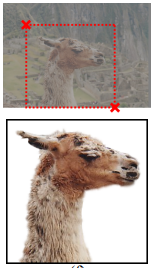
\includegraphics[width=\textwidth]{gambar/gambar-2_5(f).png}
      \caption{\emph{GrabCut}}
    \end{subfigure}  
  \caption{
    Perbandingan beberapa \emph{matting tools} dan segmentasi. (\cite{Rother:2004})
    }
  \label{img:2.5}
\end{figure}


\subsection{{Segmentasi gambar dengan algoritma \emph{GrabCut}}}

\subsubsection{{Model Pendataan Warna}}

Gambar yang ada saat ini terdiri dari piksel \(z_{n}\) dalam ruang warna RGB. 
Karena tidak praktis untuk membuat histogram ruang warna yang memadai, untuk itu 
maka digunakan GMM. Setiap nilai GMM yaitu satu untuk latar belakang dan satu untuk 
latar depan, dianggap sebagai \emph{Gaussian Mixture} penuh dengan komponen K 
(biasanya K = 5). Untuk menangani GMM dengan baik, dalam kerangka optimisasi, vektor 
tambahan \(\textbf{k} = \{k_{1},...,k_{n},...,k_{N}\}\) diperkenalkan, dengan 
\(k_{n} \in \{1,...K\}\) , menetapkan, untuk setiap piksel, komponen GMM unik, satu 
komponen baik dari latar belakang atau model latar depan, menurut \( \alpha n = 0\) 
atau \(1^1\) .


Energi Gibbs untuk segmentasi sekarang menjadi 

\begin{equation} \label{eq:rumus_energi0}
  E(\alpha,k,\theta, z) = U(\alpha,k,\theta, z) + V(\alpha, z)
\end{equation} 

bergantung juga pada variabel komponen GMM k . Istilah data U sekarang didefinisikan, 
dengan mempertimbangkan model GMM warna, sebagai 

\begin{equation} \label{eq:rumus_energi1}
  U(\alpha,k,\theta, z) =  \sum_{n} D(\alpha_{n}, k_{n},\theta,z_{n}),
\end{equation}  

di mana 

\begin{equation} \label{eq:rumus_D}
  D(\alpha n, k_{n} ,\theta,z_{n}) = - \log p(z_{n} | \alpha n, k_{n},\theta) - log \pi(\alpha_n, k_{n})
\end{equation}

yang mana \(p(\cdot)\)  adalah distribusi probabilitas Gaussian, dan \(\pi(\cdot)\) adalah 
koefisien bobot campuran, sehingga : 

\begin{multline} \label{eq:rumus_energi2}
      D(\alpha_{n}, k_{n},\theta,z_{n}) = - log \pi(\alpha_{n}, k_{n}) + \frac{1}{2} logdet \Sigma(\alpha_{n}, k_{n}) \\
      + \frac{1}{2} [z_{n} - \mu (\alpha_{n}, k_{n})]^T \Sigma(\alpha_{n}, k_{n})^{-1} [z_{n} -  \mu (\alpha n, k_{n})]    
\end{multline}

Oleh karena itu, parameter model sekarang adalah 

\begin{equation} \label{eq:rumus_energi3}
  \theta = \{ \pi(\alpha, k), \mu (\alpha, k), \Sigma (\alpha, k), \alpha = 0,1, k = 1...K \},
\end{equation}  

yaitu bobot \(\pi\), berarti \(\mu\) dan kovarians \(\Sigma\) dari komponen \(\mathcal{2K} \)
Gaussian untuk distribusi latar belakang dan latar depan. Istilah kelancaran \(\mathcal{V}\) 
pada dasarnya tidak berubah dari kasus monokrom kecuali bahwa istilah kontras dihitung 
menggunakan jarak \emph{Euclidean} dalam ruang warna: 

\begin{equation} \label{eq:rumus_energi4}
  V(\alpha, z) = \gamma \sum_{(m,n)\in C} [\alpha_{n} \neq \alpha_{m}] \textrm{ exp} - \beta \|z_{m} - z_{n}\|^2
\end{equation}


\subsubsection{{Segmentasi berdasarkan Iterasi \emph{Energy Minimization}}}


Skema minimisasi energi baru di \emph{GrabCut} bekerja secara iteratif, menggantikan algoritma 
sekali pakai sebelumnya (Boykov). Ini memiliki keuntungan yang memungkinkan 
penyempurnaan otomatis dari opasitas \(\alpha\), karena piksel berlabel baru dari 
wilayah TU pada trimap awal digunakan untuk menyempurnakan parameter GMM warna \( \theta \). 
Elemen utama dari sistem \emph{GrabCut} diberikan dalam gambar \ref{img:2.6}. Langkah 1 sangat mudah, 
dilakukan dengan pencacahan sederhana nilai kn untuk setiap piksel n. Langkah 2 
diimplementasikan sebagai satu set prosedur estimasi parameter Gaussian, sebagai 
berikut. Untuk komponen GMM k yang diberikan, katakanlah, model latar depan, himpunan 
bagian dari piksel \(F(k) = {z_{n} : k_{n} = k \: dan \: \alpha_{n} = 1}\) ditentukan. 
Rata-rata \(\mu(\alpha, k)\) dan kovarians \(\sum(\alpha, k)\) diperkirakan dengan 
cara standar sebagai rata-rata sampel dan kovarians nilai piksel dalam F(k) dan 
bobotnya adalah \(\pi(\alpha, k)= |F( k)|/\sum_{k} |F(k)|\) , di mana \(\mathcal{|S|} \)menunjukkan 
ukuran himpunan \(S\). Akhirnya langkah 3 adalah optimasi global, menggunakan \emph{minimum cut}, 
persis seperti Boykov.


Struktur algoritma menjamin sifat konvergensi yang tepat. Hal ini karena setiap 
langkah 1 sampai 3 dari minimalisasi iteratif dapat ditunjukkan sebagai minimalisasi 
energi total E sehubungan dengan tiga set variabel \(k, \theta, \alpha\) pada gilirannya. Oleh 
karena itu E berkurang secara monoton, dan ini diilustrasikan dalam praktiknya 
dalam gambar. 4. Dengan demikian algoritma dijamin konvergen setidaknya ke minimum 
lokal E. Sangat mudah untuk mendeteksi kapan E berhenti menurun secara signifikan, 
dan menghentikan iterasi secara otomatis. 


Manfaat praktis dari minimisasi iteratif. Gambar. \ref{img:2.5}(e) dan \ref{img:2.5}(f) 
mengilustrasikan bagaimana kekuatan tambahan dari minimisasi iteratif dalam 
\emph{Grab Cut} dapat sangat mengurangi jumlah interaksi pengguna yang diperlukan 
untuk menyelesaikan tugas segmentasi, relatif terhadap pendekatan \emph{one-shot graph cut}. 
Ini terlihat dalam dua cara. Pertama, tingkat pengeditan pengguna yang diperlukan, 
setelah inisialisasi dan pengoptimalan, dikurangi. Kedua, interaksi awal bisa lebih 
sederhana, misalnya dengan mengizinkan pelabelan yang tidak lengkap oleh pengguna.

\begin{figure}[H]
  \centering
    \begin{subfigure}{0.5\textwidth}
      \centering{}
      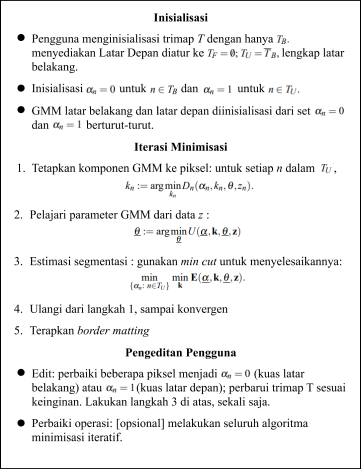
\includegraphics[width=\textwidth]{gambar/gambar-2_6.png}
    \end{subfigure}     
  \caption{
    Segmentasi gambar di \emph{GrabCut} (\cite{Rother:2004})
    }
  \label{img:segmentasi_grabcut}
\end{figure}


\begin{figure}[H]
  \centering
    \begin{subfigure}{0.3\textwidth}
      \centering{}
      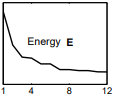
\includegraphics[width=\textwidth]{gambar/gambar-2_7(a).png}
      \caption{}
    \end{subfigure}%
    \begin{subfigure}{0.3\textwidth}
      \centering{}
      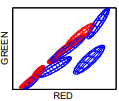
\includegraphics[width=\textwidth]{gambar/gambar-2_7(b).png}
      \caption{}
    \end{subfigure}  
    \begin{subfigure}{0.3\textwidth}
      \centering{}
      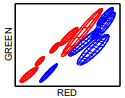
\includegraphics[width=\textwidth]{gambar/gambar-2_7(c).png}
      \caption{}
    \end{subfigure}  
  \caption{
    Konvergensi minimalisasi iteratif untuk data gambar \ref{img:2.5}(f). (a) Energi E untuk contoh 
    llama konvergen selama 12 iterasi dengan K = 5, komponen campuran digunakan untuk latar belakang (merah) dan latar depan (biru) (\cite{Rother:2004}). 
    }
    \label{img:2.7}
\end{figure}

\subsubsection{{Interaksi Pengguna dan Trimap yang Tidak Lengkap}}

\textbf{Trim tidak lengkap}. Algoritma minimisasi iteratif memungkinkan peningkatan 
keserbagunaan interaksi pengguna. Secara khusus, pelabelan yang tidak lengkap menjadi 
layak di mana, sebagai pengganti trimap T penuh, pengguna hanya perlu menentukan, 
katakanlah, wilayah latar belakang \(T_{B}\), meninggalkan \(T_{F} = 0\). Tidak ada pelabelan latar 
depan keras yang dilakukan sama sekali. Minimisasi iteratif (gambar \ref{img:2.6}) menangani 
ketidaklengkapan ini dengan mengizinkan label sementara pada beberapa piksel (di 
latar depan) yang kemudian dapat ditarik kembali; hanya label latar belakang \(T_{B}\) 
yang dianggap tegas — dijamin tidak akan ditarik kembali nantinya. (Tentu saja 
skema pelengkap, dengan label tegas untuk latar depan saja, juga memungkinkan.) 
\(T_{B}\) awal ditentukan oleh pengguna sebagai strip piksel di sekitar bagian 
luar sudut persegi yang ditandai ( ditandai dengan warna merah pada gambar \ref{img:2.5}(f))

\begin{figure}[H]
  \centering
    \begin{subfigure}{0.5\textwidth}
      \centering{}
      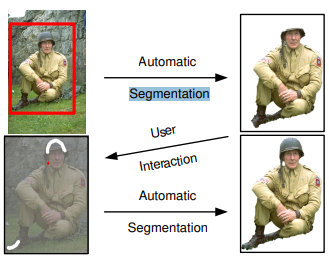
\includegraphics[width=\textwidth]{gambar/gambar-2_8.png}
    \end{subfigure}     
  \caption{
    Pengeditan pengguna. Setelah interaksi pengguna awal dan segmentasi (baris atas), 
    pengeditan pengguna lebih lanjut (gambar \ref{img:2.6}) diperlukan. (\cite{Rother:2004})
    }
    \label{img:2.8}
\end{figure}

\textbf{Pengeditan pengguna lebih lanjut.} Pelabelan pengguna awal yang tidak lengkap 
cukup sepuluh untuk memungkinkan seluruh segmentasi diselesaikan secara otomatis, 
tetapi tidak berarti selalu. Jika tidak, pengeditan pengguna lebih lanjut diperlukan, 
seperti yang ditunjukkan pada gambar \ref{img:2.8}. Ini mengambil bentuk menyikat piksel, membatasinya 
menjadi latar depan yang kokoh atau latar belakang yang kokoh; lalu minimisasi 
langkah 3. pada gambar \ref{img:2.6} diterapkan. Perhatikan bahwa cukup menyikat, secara 
kasar, hanya sebagian dari area yang salah diberi label. Selain itu, operasi "perbaiki" 
opsional dari gambar \ref{img:2.6} memperbarui model warna, mengikuti suntingan pengguna. Ini 
menopang efek operasi edit yang seringkali bermanfaat. Perhatikan bahwa untuk efisiensi 
aliran optimal, dihitung dengan \emph{graph cut}, dapat digunakan kembali selama 
pengeditan pengguna.

